\section{Базовые строковые алгоритмы}

\subsection{Задача о вхождении шаблона в текст}

Договоримся сначала о базовых понятиях. С теоретической точки зрения \textit{строка} $s$ длины $n$ "--- это конечная последовательность символов $s_0 s_1 \dots s_{n-1}$ (индексация всегда с нуля), каждый из которых берётся из некоторого фиксированного алфавита $\Sigma$. Длину строки $s$ будем обозначать через $|s|$.

Почти везде нам будет достаточно следующей простой модели: алфавит $\Sigma$ конечен и имеет константный размер. Классический пример "--- строчные латинские буквы:
\[
    \Sigma = \{\text{\texttt{'a'}}, \text{\texttt{'b'}}, \text{\texttt{'c'}}, \dots, \text{\texttt{'z'}}\}, \qquad |\Sigma| = 26.
\]
Такому алфавиту естественным образом сопоставляются числа от $1$ до $26$. На практике строки в C++ хранятся как последовательности элементов типа \texttt{char}, у которого область значений тоже совсем маленькая ($256$ вариантов), так что между $26$ и $256$ принципиальной разницы нет. В некоторых будущих алгоритмах константность размера алфавита будет существенна, но в сегодняшней лекции почти везде можно считать алфавит произвольным.

Начнём с классической задачи, которая возникает всякий раз, когда вы нажимаете \texttt{Ctrl+F} в текстовом редакторе.

\begin{problem}[о вхождении шаблона в текст]
    Даны две строки: короткий шаблон $p$ и длинный текст $t$. Требуется найти все вхождения строки $p$ в строку $t$ в качестве подстроки, то есть указать все такие позиции в $t$, начиная с которых подстрока длины $|p|$ посимвольно совпадает с $p$.
\end{problem}

\begin{center}
\begin{tikzpicture}[scale=0.95]
    % Шаблон p
    \draw[thick, fill=blue!8] (0, 1.1) rectangle (2.6, 1.6);
    \node[above] at (1.3, 1.6) {$p$};
    \draw[decorate, decoration={brace, mirror, amplitude=4pt}] (0, 1.0) -- (2.6, 1.0);

    % Текст t
    \draw[thick] (4.0, 1.1) rectangle (12.5, 1.6);
    \node[above] at (8.25, 1.6) {$t$};
    \draw[thick, fill=blue!8] (6.2, 1.1) rectangle (8.8, 1.6);
    \draw[decorate, decoration={brace, mirror, amplitude=4pt}] (6.2, 1.0) -- (8.8, 1.0)
        node[midway, below=4pt] {\small совпадение с $p$};
\end{tikzpicture}
\end{center}

Наивный способ решения очевиден: приложим шаблон $p$ ко всем возможным стартовым позициям в тексте $t$ и для каждой из них честно проверим посимвольное совпадение. Поскольку проверка одной позиции требует $O(|p|)$ сравнений, в худшем случае такое решение работает за $O(|p| \cdot |t|)$. Если обе строки имеют длину порядка $10^6$, это квадратичное время, которое никуда не годится. Разберём несколько подходов, позволяющих решать эту задачу за линейное время $O(|p| + |t|)$.

\subsection{Полиномиальное хеширование и алгоритм Рабина--Карпа}

Первая техника "--- полиномиальное хеширование. Идея простая: вместо того чтобы сравнивать строки посимвольно за время, пропорциональное их длине, сопоставим каждой строке некоторое число (её \textit{хеш}) из небольшого диапазона, помещающегося в стандартный целочисленный тип данных. Тогда сравнение двух строк сведётся к сравнению двух чисел за $O(1)$. Разумеется, поскольку разных строк гораздо больше, чем возможных значений хеша, неизбежны \textit{коллизии} "--- ситуации, когда у разных строк хеши совпали. Наша цель "--- сделать вероятность такой ошибки пренебрежимо малой.

\begin{definition}
    Пусть $s = s_0 s_1 \dots s_{n-1}$ "--- строка длины $n$, где каждый символ $s_i$ заменён своим числовым кодом (номером буквы в алфавите или ASCII-кодом). Зафиксируем целое основание $b$ и простой модуль $m$. \textit{Полиномиальным хешем} строки $s$ назовём величину
    \begin{equation}\label{eq:poly_hash}
        h(s) = \bigl(s_0 b^{n-1} + s_1 b^{n-2} + \dots + s_{n-2} b + s_{n-1}\bigr) \bmod m.
    \end{equation}
\end{definition}

\begin{note}
    Критически важно, чтобы \textbf{никакой символ алфавита не кодировался нулём} ($s_i \ne 0$). Именно поэтому мы нумеруем буквы латинского алфавита числами от $1$ до $26$, а не с нуля. Если бы символ \texttt{'a'} имел код $0$, то строки \texttt{"a"} и \texttt{"aa"} при любых $b$ и $m$ имели бы один и тот же хеш:
    \[
        h(\text{\texttt{"a"}}) = 0, \qquad h(\text{\texttt{"aa"}}) = (0 \cdot b + 0) \bmod m = 0,
    \]
    то есть давали бы гарантированную коллизию. Требование $s_i \ne 0$ обеспечивает нетривиальность старшего коэффициента многочлена \eqref{eq:poly_hash}.
\end{note}

Поймём, почему при случайном выборе основания $b$ коллизии происходят редко. Будем считать, что простой модуль $m$ фиксирован заранее (он является частью определения хеш-функции), а основание $b$ выбирается случайно и равновероятно из множества $\{0, 1, \dots, m - 1\}$, то есть все вычисления происходят в поле вычетов $\Z_m$.

\begin{proposition}[оценка вероятности коллизии]
    Пусть $m$ "--- простое число, а $b$ выбирается равновероятно из $\Z_m$. Для любых двух строк $p$ и $s$:
    \begin{enumerate}
        \item если $p = s$, то $h(p) = h(s)$ с вероятностью $1$;
        \item если $p \ne s$, то вероятность коллизии не превосходит
        \[
            \Prob_b\bigl(h(s) = h(p)\bigr) \le \frac{\max(|s|, |p|)}{m}.
        \]
    \end{enumerate}
\end{proposition}

\begin{proof}
    Первое свойство очевидно: у одинаковых строк на одних и тех же местах стоят одинаковые символы, поэтому выражения \eqref{eq:poly_hash} совпадают.

    Докажем второе свойство. Пусть $p \ne s$. Не умаляя общности, будем считать, что $|s| \ge |p|$, и обозначим $n = |s| = \max(|s|, |p|)$. Если строка $p$ короче $s$, припишем к многочлену $h(p)$ слева недостающие старшие степени $b$ с нулевыми коэффициентами $p_k = 0$ (значение хеша $h(p)$ от этого не изменится). Тогда условие коллизии $h(s) = h(p)$ переписывается как сравнение по модулю $m$:
    \[
        s_0 b^{n-1} + s_1 b^{n-2} + \dots + s_{n-1} \equiv p_0 b^{n-1} + p_1 b^{n-2} + \dots + p_{n-1} \pmod m.
    \]
    Перенесём все слагаемые в левую часть:
    \begin{equation}\label{eq:poly_diff}
        (s_0 - p_0) b^{n-1} + (s_1 - p_1) b^{n-2} + \dots + (s_{n-1} - p_{n-1}) \equiv 0 \pmod m.
    \end{equation}
    Рассмотрим левую часть \eqref{eq:poly_diff} как многочлен от переменной $b$ над полем $\Z_m$ (напомним, что $m$ "--- простое число, поэтому $\Z_m$ является полем). Поскольку строки $p$ и $s$ различны, а все настоящие символы кодируются ненулевыми числами, хотя бы одна скобка $(s_k - p_k)$ отлична от нуля (если $|s| = |p|$, строки отличаются в каком-то разряде; если же $|s| > |p|$, то $p_0 = 0$, тогда как $s_0 \ne 0$). Значит, это ненулевой многочлен степени не выше $n - 1$.

    Ненулевой многочлен степени не выше $n - 1$ над полем $\Z_m$ имеет не более $n - 1$ корней. Всего возможных точек $b \in \Z_m$ ровно $m$, а <<плохих>> точек, в которых происходит коллизия, не более $n - 1$. Следовательно,
    \[
        \Prob_b\bigl(h(s) = h(p)\bigr) \le \frac{n - 1}{m} \le \frac{\max(|s|, |p|)}{m}. \qedhere
    \]
\end{proof}

Таким образом, если $h(p) = h(s)$, мы можем с большой уверенностью считать, что $p = s$. Например, при длине строк порядка $10^6$ и простом модуле $m \approx 10^9$ вероятность коллизии двух фиксированных строк не превышает $10^6 / 10^9 = 10^{-3}$. Если хочется уменьшить вероятность ошибки до микроскопических величин, есть два стандартных пути:
\begin{itemize}
    \item взять модуль побольше (например, $m \approx 10^{18}$, используя $64$-битные/128-битные типы данных);
    \item считать хеши параллельно по нескольким простым модулям $m_1, m_2, m_3, m_4$ со своими независимыми основаниями $b_1, b_2, b_3, b_4$ и объявлять строки равными только тогда, когда совпали все четыре хеша.
\end{itemize}

\subsubsection*{Хеши подстрок и алгоритм Рабина--Карпа}

Вернёмся к задаче поиска шаблона $p$ в тексте $t$. Мы можем один раз посчитать $h(p)$ за $O(|p|)$, а затем сравнивать его с хешами всех подстрок текста $t$ длины $|p|$. Осталось научиться быстро находить хеш произвольной подстроки $t[l \dots r] = t_l t_{l+1} \dots t_r$.

Применим трюк в духе префиксных сумм. Предпосчитаем \textit{префиксные хеши} текста $t$:
\[
    \pref_i = h(t_0 t_1 \dots t_i), \qquad i = 0, 1, \dots, |t| - 1.
\]
База очевидна: $\pref_0 = t_0 \bmod m$. Посмотрим, как пересчитать $\pref_i$ через $\pref_{i-1}$. Когда мы дописываем в конец строки $t_0 \dots t_{i-1}$ один новый символ $t_i$, все старые символы в формуле \eqref{eq:poly_hash} сдвигаются на одну позицию влево, то есть степень $b$ при каждом из них увеличивается ровно на единицу, а в конец добавляется свободный член $t_i$. Значит,
\[
    \pref_i = (\pref_{i-1} \cdot b + t_i) \bmod m.
\]
Весь массив $\pref$ насчитывается слева направо за $O(|t|)$.

Теперь выразим хеш подстроки $t[l \dots r]$ (при $l \ge 1$; случай $l = 0$ тривиален, так как $h(t[0 \dots r]) = \pref_r$).

\begin{center}
\begin{tikzpicture}[scale=0.95]
    % Полоска строки t
    \draw[thick] (0, 0) rectangle (12.5, 0.6);
    \node[left] at (-0.2, 0.3) {$t$:};

    % Заштрихованный префикс 0..l-1
    \fill[pattern=north east lines, pattern color=red!60] (0, 0) rectangle (4.8, 0.6);
    \draw[thick] (4.8, 0) -- (4.8, 0.6);

    % Подстрока l..r
    \fill[blue!12] (4.8, 0) rectangle (9.6, 0.6);
    \draw[thick] (9.6, 0) -- (9.6, 0.6);

    % Подписи индексов
    \node[below] at (0, 0) {\small $0$};
    \node[below] at (4.2, 0) {\small $l-1$};
    \node[below] at (5.05, 0) {\small $l$};
    \node[below] at (9.6, 0) {\small $r$};

    % Дужки сверху и снизу
    \draw[decorate, decoration={brace, amplitude=6pt}, thick] (0, 0.7) -- (9.6, 0.7)
        node[midway, above=6pt] {$\pref_r$: степени $b$ от $b^r$ до $b^0$};

    \draw[decorate, decoration={brace, mirror, amplitude=5pt}, thick, red!75!black] (0, -0.55) -- (4.75, -0.55)
        node[midway, below=5pt] {$\pref_{l-1} \cdot b^{r-l+1}$};

    \draw[decorate, decoration={brace, mirror, amplitude=5pt}, thick, blue!75!black] (4.85, -0.55) -- (9.6, -0.55)
        node[midway, below=5pt] {$h(t[l \dots r])$ (длина $r - l + 1$)};
\end{tikzpicture}
\end{center}

Посмотрим на многочлен $\pref_r = h(t_0 \dots t_r)$. Последние $r - l + 1$ его слагаемых (от $t_l b^{r-l}$ до $t_r b^0$) идут ровно с теми коэффициентами и степенями $b$, которые нужны в $h(t[l \dots r])$. Нам мешают только первые $l$ слагаемых, отвечающих префиксу $t_0 \dots t_{l-1}$. В выражении $\pref_{l-1}$ эти самые символы уже сложены со степенями $b^{l-1}, \dots, b^1, b^0$, а в $\pref_r$ они входят со степенями $b^r, \dots, b^{r-l+1}$, то есть ровно в $b^{r-l+1}$ раз большими. Поэтому достаточно домножить $\pref_{l-1}$ на $b^{r-l+1}$ и вычесть из $\pref_r$:
\begin{equation}\label{eq:substring_hash}
    h(t[l \dots r]) = \bigl(\pref_r - \pref_{l-1} \cdot b^{r - l + 1}\bigr) \bmod m.
\end{equation}
(В реализации на C++ не забываем прибавить $m$ перед взятием остатка, чтобы результат вычитания не стал отрицательным.)

Если заранее за $O(|t|)$ предпосчитать все степени основания $b^0, b^1, \dots, b^{|t|} \pmod m$, то по формуле \eqref{eq:substring_hash} хеш любой подстроки вычисляется за $O(1)$. Это сразу даёт \textbf{алгоритм Рабина--Карпа}:
\begin{enumerate}
    \item Насчитываем $h(p)$ за $O(|p|)$, а также префиксные хеши $\pref_i$ текста $t$ и степени $b^k \bmod m$ за $O(|t|)$.
    \item Перебираем все подстроки текста $t$ длины $|p|$ и за $O(1)$ сравниваем хеш каждой из них с $h(p)$. Если хеши совпали "--- объявляем, что нашли вхождение.
\end{enumerate}
Итоговое время работы алгоритма Рабина--Карпа составляет $O(|p| + |t|)$.

\subsection{Префикс-функция}

Полиномиальные хеши очень удобны на практике, но у них есть теоретический изъян "--- ненулевая вероятность ошибки и необходимость источника случайности. Построим теперь полностью детерминированные линейные алгоритмы решения той же задачи. Первый из них основан на префикс-функции.

\begin{definition}
    Пусть $s = s_0 s_1 \dots s_{n-1}$ "--- строка длины $n$. \textit{Префикс-функцией} строки $s$ называется массив из $n$ чисел $\pi_0, \pi_1, \dots, \pi_{n-1}$, где $\pi_i$ "--- длина максимального собственного суффикса подстроки $s[0 \dots i] = s_0 \dots s_i$, совпадающего с её префиксом той же длины.
\end{definition}

Для краткости подстроку, которая одновременно является собственным суффиксом и префиксом рассматриваемой строки, будем называть \textit{супрефиксом} (или \textit{собственным супрефиксом}). Иными словами, для каждого $i$ мы оставляем от строки $s$ только начальный кусок $s_0 \dots s_i$ и ищем у него самый длинный собственный супрефикс "--- его длина и есть $\pi_i$.

\begin{center}
\begin{tikzpicture}[scale=0.95]
    \draw[thick] (0, 0) rectangle (7.5, 0.55);
    \fill[pattern=north east lines, pattern color=blue!60] (0, 0) rectangle (2.6, 0.55);
    \fill[pattern=north east lines, pattern color=blue!60] (4.9, 0) rectangle (7.5, 0.55);
    \draw[thick] (2.6, 0) -- (2.6, 0.55);
    \draw[thick] (4.9, 0) -- (4.9, 0.55);

    \node[below] at (0, 0) {$s_0$};
    \node[below] at (7.5, 0) {$s_i$};

    \draw[decorate, decoration={brace, amplitude=5pt}, thick] (0, 0.65) -- (2.6, 0.65)
        node[midway, above=4pt] {$\pi_i$};
    \draw[decorate, decoration={brace, amplitude=5pt}, thick] (4.9, 0.65) -- (7.5, 0.65)
        node[midway, above=4pt] {$\pi_i$};
\end{tikzpicture}
\end{center}

Слово <<собственный>> означает, что вся строка $s_0 \dots s_i$ целиком не годится (иначе определение было бы тривиальным: вся строка всегда равна самой себе, и мы бы получили $\pi_i = i + 1$). Нас же интересует максимальный нетривиальный супрефикс длины строго меньше $i + 1$.

Отметим сразу, что $\pi_0 = 0$ всегда. В самом деле, при $i = 0$ мы рассматриваем одноэлементную строку $s_0$. У неё всего два суффикса: вся строка $s_0$ (не собственный) и пустая строка $\epsilon$ длины $0$, которая совпадает с пустым префиксом.

\subsubsection*{Решение задачи о вхождении шаблона в текст}

Предположим пока, что у нас есть <<чёрный ящик>>, умеющий за линейное время вычислять префикс-функцию любой строки. Покажем, как за $O(|p| + |t|)$ найти все вхождения шаблона $p$ в текст $t$.

Склеим строки $p$ и $t$ через специальный разделительный символ $\text{\texttt{'\#'}}$:
\[
    s = p + \text{\texttt{'\#'}} + t,
\]
где $\text{\texttt{'\#'}}$ "--- новый (<<свежий>>) символ, который гарантированно не встречается ни в $p$, ни в $t$.

\begin{center}
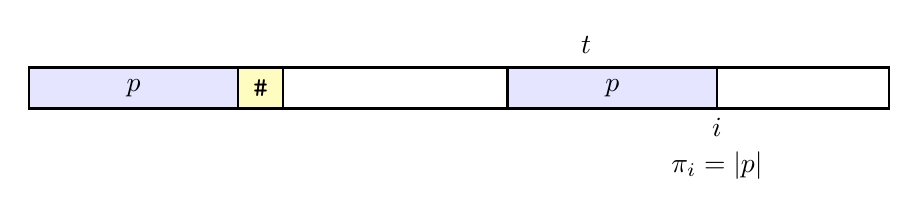
\begin{tikzpicture}[scale=0.95]
    \draw[thick, fill=blue!10] (0, 0) rectangle (2.8, 0.55);
    \node at (1.4, 0.275) {$p$};

    \draw[thick, fill=yellow!25] (2.8, 0) rectangle (3.4, 0.55);
    \node at (3.1, 0.275) {\texttt{\#}};

    \draw[thick] (3.4, 0) rectangle (11.5, 0.55);
    \node[above] at (7.45, 0.6) {$t$};

    \draw[thick, fill=blue!10] (6.4, 0) rectangle (9.2, 0.55);
    \node at (7.8, 0.275) {$p$};
    \node[below] at (9.2, 0) {$i$};
    \node[below] at (9.2, -0.45) {$\pi_i = |p|$};
\end{tikzpicture}
\end{center}

\begin{proposition}
    В строке $s = p + \text{\texttt{'\#'}} + t$ для всех позиций $i$ выполнено $\pi_i \le |p|$. При этом равенство $\pi_i = |p|$ достигается тогда и только тогда, когда в позиции $i$ заканчивается очередное вхождение шаблона $p$ в текст $t$.
\end{proposition}

\begin{proof}
    Поймём сначала, почему не бывает $\pi_i > |p|$. Если бы в некоторой позиции $i$ нашёлся собственный супрефикс длины строго больше $|p|$, то соответствующий префикс строки $s$ содержал бы $(|p| + 1)$-й символ, то есть разделитель $\text{\texttt{'\#'}}$. Но префикс равен суффиксу, а значит, символ $\text{\texttt{'\#'}}$ должен был бы встретиться где-то правее в строке $t$, что невозможно по выбору разделителя.

    Следовательно, $\pi_i \le |p|$ всегда. Равенство же $\pi_i = |p|$ при $i > |p|$ в точности означает, что суффикс строки $s[0 \dots i]$ длины $|p|$ совпадает с префиксом $s$ длины $|p|$, то есть с шаблоном $p$. И наоборот: если в позиции $i$ заканчивается вхождение $p$, то суффикс длины $|p|$ равен $p$, а поскольку больше $|p|$ значение префикс-функции быть не может, получаем $\pi_i = |p|$.
\end{proof}

\subsubsection*{Алгоритм вычисления префикс-функции}

Научимся теперь находить массив $\pi_0, \pi_1, \dots, \pi_{n-1}$ для произвольной строки $s$ длины $n$. Будем идти по строке слева направо: $\pi_0 = 0$ уже известно, и на шаге $i$ ($1 \le i \le n - 1$) мы хотим вычислить $\pi_i$, опираясь на все предыдущие значения $\pi_0, \dots, \pi_{i-1}$.

Договоримся о терминологии на фиксированном шаге $i$: префикс $s[0 \dots i-1]$ будем называть \textit{старой} строкой, а префикс $s[0 \dots i]$ (полученный дописыванием символа $s_i$ справа) "--- \textit{новой} строкой. Нас интересует максимальный собственный супрефикс новой строки.

\begin{center}
\begin{tikzpicture}[scale=0.95]
    % Старая строка
    \node[left] at (-0.3, 1.4) {\small старая строка:};
    \draw[thick] (0, 1.15) rectangle (8.0, 1.65);
    \fill[pattern=north east lines, pattern color=blue!60] (0, 1.15) rectangle (2.5, 1.65);
    \fill[pattern=north east lines, pattern color=blue!60] (5.5, 1.15) rectangle (8.0, 1.65);
    \draw[thick] (2.5, 1.15) -- (2.5, 1.65);
    \draw[thick] (5.5, 1.15) -- (5.5, 1.65);
    \node[below] at (0, 1.15) {\small $0$};
    \node[below] at (7.8, 1.15) {\small $i-1$};

    % Новая строка
    \node[left] at (-0.3, 0.1) {\small новая строка:};
    \draw[thick] (0, -0.15) rectangle (8.0, 0.35);
    \draw[thick, fill=orange!20] (8.0, -0.15) rectangle (8.6, 0.35);
    \fill[pattern=north east lines, pattern color=blue!60] (0, -0.15) rectangle (2.5, 0.35);
    \draw[thick, fill=orange!20] (2.5, -0.15) rectangle (3.1, 0.35);
    \fill[pattern=north east lines, pattern color=blue!60] (5.5, -0.15) rectangle (8.0, 0.35);
    \draw[thick] (5.5, -0.15) -- (5.5, 0.35);

    \node[below] at (0, -0.15) {\small $0$};
    \node[below] at (2.8, -0.15) {\small $s_j$};
    \node[below] at (7.6, -0.15) {\small $i-1$};
    \node[below] at (8.3, -0.15) {\small $s_i$};
\end{tikzpicture}
\end{center}

Сделаем ключевое наблюдение: если взять максимальный собственный супрефикс новой строки (при $\pi_i > 0$) и отбросить от него последний символ $s_i$, то оставшийся кусок длины $\pi_i - 1$ обязательно будет собственным супрефиксом \textit{старой} строки! Действительно, мы от двух равных строк (префикса и суффикса новой строки) отбросили по одному последнему символу "--- оставшиеся префикс и суффикс старой строки по-прежнему равны.

Отсюда возникает естественная идея алгоритма:
\begin{quote}
    \textit{Будем перебирать все собственные супрефиксы старой строки в порядке убывания их длины и остановимся в первый момент, когда префикс и суффикс продлеваются направо одним и тем же символом (то есть когда символ после префикса совпадает с $s_i$).}
\end{quote}

Поймём, как организовать такой перебор. Введём переменную $j$ "--- длину текущего рассматриваемого супрефикса старой строки.
\begin{enumerate}
    \item С чего начать перебор? По определению префикс-функции самый длинный собственный супрефикс старой строки $s[0 \dots i-1]$ имеет длину $j = \pi_{i-1}$.
    \item Как проверить, продлевается ли супрефикс длины $j$ новым символом $s_i$? Префикс длины $j$ занимает позиции $0, 1, \dots, j - 1$, поэтому сразу за ним стоит символ $s_j$. Значит, условие продления имеет вид $s_i = s_j$. Если оно выполнено, то $\pi_i = j + 1$, и перебор окончен.
    \item Как перейти к следующему по длине супрефиксу старой строки, если $s_i \ne s_j$?
\end{enumerate}

Разберём третий пункт подробнее. Пусть у нас есть текущий супрефикс старой строки длины $j$, и мы ищем следующий по величине (чуть более короткий) супрефикс старой строки.

\begin{center}
\begin{tikzpicture}[scale=0.95]
    \draw[thick] (0, 0) rectangle (11, 0.55);

    % Большой супрефикс длины j
    \draw[decorate, decoration={brace, amplitude=7pt}, thick, blue!70!black] (0, 0.65) -- (4.5, 0.65)
        node[midway, above=6pt] {$j$};
    \draw[decorate, decoration={brace, amplitude=7pt}, thick, blue!70!black] (6.5, 0.65) -- (11, 0.65)
        node[midway, above=6pt] {$j$};

    \draw[thick, blue!70!black] (4.5, 0) -- (4.5, 0.55);
    \draw[thick, blue!70!black] (6.5, 0) -- (6.5, 0.55);

    % Меньший супрефикс внутри них
    \fill[pattern=north east lines, pattern color=teal!80!black] (0, 0) rectangle (1.8, 0.55);
    \fill[pattern=north east lines, pattern color=teal!80!black] (2.7, 0) rectangle (4.5, 0.55);
    \fill[pattern=north east lines, pattern color=teal!80!black] (9.2, 0) rectangle (11, 0.55);

    \draw[thick] (1.8, 0) -- (1.8, 0.55);
    \draw[thick] (2.7, 0) -- (2.7, 0.55);
    \draw[thick] (9.2, 0) -- (9.2, 0.55);

    \draw[decorate, decoration={brace, mirror, amplitude=5pt}, thick, teal!70!black] (0, -0.1) -- (1.8, -0.1)
        node[midway, below=4pt] {$\pi_{j-1}$};
    \draw[decorate, decoration={brace, mirror, amplitude=5pt}, thick, teal!70!black] (2.7, -0.1) -- (4.5, -0.1)
        node[midway, below=4pt] {$\pi_{j-1}$};
    \draw[decorate, decoration={brace, mirror, amplitude=5pt}, thick, teal!70!black] (9.2, -0.1) -- (11, -0.1)
        node[midway, below=4pt] {$\pi_{j-1}$};
\end{tikzpicture}
\end{center}

Посмотрим на рисунок. Искомый меньший супрефикс старой строки (заштрихованные участки в самом начале и в самом конце) имеет длину меньше $j$, поэтому правый заштрихованный участок целиком лежит внутри суффикса длины $j$. Но суффикс старой строки длины $j$ посимвольно равен её префиксу длины $j$! Значит, мы можем перенести правую дужку в конец префикса длины $j$ (на участок, заканчивающийся в позиции $j - 1$).

Получается, что любой супрефикс старой строки длины меньше $j$ одновременно является собственным супрефиксом префикса $s[0 \dots j-1]$ длины $j$ (и наоборот). Нам нужен самый длинный из них, а максимальный собственный супрефикс строки $s[0 \dots j-1]$ по определению имеет длину $\pi_{j-1}$. Тем самым переход к следующему по длине супрефиксу записывается одной формулой:
\[
    j \gets \pi_{j-1}.
\]

Осталось аккуратно выписать код. Назовём массив префикс-функции \texttt{p}:

\begin{lstlisting}
string s;
int n = s.size();
vector<int> p(n, 0);
int j = 0;
for (int i = 1; i < n; ++i) {
    // в этот момент j == p[i - 1]
    while (j > 0 && s[i] != s[j]) {
        j = p[j - 1]; // переходим к следующему по длине супрефиксу
    }
    if (s[i] == s[j]) {
        ++j;
    }
    p[i] = j;
}
\end{lstlisting}

Обратите внимание на выход из цикла \texttt{while}: мы выходим из него либо когда нашли супрефикс, который продлевается символом $s_i = s_j$ (и тогда \texttt{if} увеличивает $j$ на единицу), либо когда дошли до пустого супрефикса $j = 0$. Если даже пустой супрефикс не продлевается ($s_i \ne s_0$), условие в \texttt{if} не срабатывает, и в \texttt{p[i]} записывается $0$, как и должно быть. Заметим также, что инвариант \texttt{j == p[i - 1]} в начале тела цикла \texttt{for} поддерживается автоматически, поскольку в конце предыдущей итерации мы выполнили \texttt{p[i - 1] = j}.

\begin{theorem}
    Приведённый алгоритм вычисляет префикс-функцию строки длины $n$ за время $O(n)$.
\end{theorem}

\begin{proof}
    Единственное место, которое могло бы работать долго "--- внутренний цикл \texttt{while}, поскольку на отдельном шаге $i$ он может сделать много итераций. Оценим суммарное число итераций цикла \texttt{while} за всё время работы алгоритма, проследив за значением переменной $j$.

    Заметим три факта:
    \begin{enumerate}
        \item Всякий раз переменной $j$ хранится длина некоторого супрефикса, поэтому $j \ge 0$ в любой момент времени (и изначально $j = 0$).
        \item Переменная $j$ увеличивается только в строчке \texttt{++j} внутри условного оператора \texttt{if}, который срабатывает не более одного раза за одну итерацию внешнего цикла \texttt{for}. Значит, за все $n - 1$ итераций цикла \texttt{for} переменная $j$ суммарно увеличится не более чем на $n - 1$.
        \item На каждой итерации цикла \texttt{while} присваивание \texttt{j = p[j - 1]} переходит от супрефикса длины $j$ к собственному супрефиксу меньшей длины $\pi_{j-1} < j$, то есть строго уменьшает целочисленную переменную $j$ хотя бы на $1$.
    \end{enumerate}
    Поскольку неотрицательная величина $j$ суммарно выросла не более чем на $n - 1$, она не может уменьшиться на единицу более чем $n - 1$ раз. Следовательно, суммарное количество итераций цикла \texttt{while} за весь алгоритм не превосходит $n$, и общее время работы составляет $O(n)$.
\end{proof}

\begin{note}
    Возня с суффиксами, совпадающими с какими-то префиксами, будет сопровождать нас на протяжении почти всех строковых лекций "--- и в алгоритме Ахо--Корасик, и в суффиксном массиве, и в суффиксном дереве с суффиксным автоматом. Поэтому префикс-функция "--- отличная разминка перед более сложными структурами.
\end{note}

\subsection{Z-функция}

Разберём ещё один линейный детерминированный подход к задаче о вхождении шаблона в текст, который смотрит на строку <<с другой стороны>>.

\begin{definition}
    Пусть $s = s_0 s_1 \dots s_{n-1}$ "--- строка длины $n$. Её \textit{Z-функцией} называется массив из $n$ чисел $z_0, z_1, \dots, z_{n-1}$, где при $i \ge 1$ величина
    \[
        z_i = \max \bigl\{k \in [0, n - i] \;\big|\; s_0 \dots s_{k-1} = s_i \dots s_{i+k-1}\bigr\}
    \]
    равна длине максимального общего префикса всей строки $s$ и её суффикса, начинающегося в позиции $i$. Значение $z_0$ по определению полагаем равным $0$.
\end{definition}

Почему мы отдельно доопределяем $z_0 = 0$? Формально при $i = 0$ наибольшая подстрока с началом в нуле, совпадающая с префиксом "--- это вся строка $s$ длины $n$. Но число $n$ никакой новой информации не несёт, а в коде гораздо удобнее считать $z_0 = 0$, чтобы не писать лишних условий.

\begin{center}
\begin{tikzpicture}[scale=0.95]
    \draw[thick] (0, 0) rectangle (10.5, 0.55);
    \fill[pattern=north east lines, pattern color=blue!60] (0, 0) rectangle (2.8, 0.55);
    \fill[pattern=north east lines, pattern color=blue!60] (4.8, 0) rectangle (7.6, 0.55);
    \draw[thick] (2.8, 0) -- (2.8, 0.55);
    \draw[thick] (4.8, 0) -- (4.8, 0.55);
    \draw[thick] (7.6, 0) -- (7.6, 0.55);

    \node[below] at (0, 0) {$0$};
    \node[below] at (4.8, 0) {$i$};

    \draw[decorate, decoration={brace, amplitude=5pt}, thick] (0, 0.65) -- (2.8, 0.65)
        node[midway, above=4pt] {$z_i$};
    \draw[decorate, decoration={brace, amplitude=5pt}, thick] (4.8, 0.65) -- (7.6, 0.65)
        node[midway, above=4pt] {$z_i$};
\end{tikzpicture}
\end{center}

Сравним геометрический смысл двух функций: если мы встали в позицию $i$, то префикс-функция $\pi_i$ ищет максимальное <<крыло влево>> (суффикс с концом в $i$), равное префиксу строки, а Z-функция $z_i$ ищет максимальное <<крыло вправо>> (подстроку с началом в $i$), равное префиксу строки. Подстроку длины $z_i$, начинающуюся в позиции $i$ (и равную префиксу той же длины), будем для удобства называть \textit{Z-блоком} с началом в $i$.

\subsubsection*{Решение задачи о вхождении шаблона в текст}

Если мы умеем находить Z-функцию за линейное время, задача поиска шаблона $p$ в тексте $t$ решается совершенно аналогично префикс-функции:
\begin{enumerate}
    \item Составляем строку $s = p + \text{\texttt{'\#'}} + t$ и вычисляем для неё массив $z$.
    \item За счёт свежего разделителя $\text{\texttt{'\#'}}$ ни при каком $i > |p|$ значение $z_i$ не может превысить $|p|$ (иначе где-то правее в $t$ нашёлся бы ещё один символ $\text{\texttt{'\#'}}$).
    \item В каждой позиции $i > |p|$, где $z_i = |p|$, в точности \textbf{начинается} очередное вхождение шаблона $p$ в текст $t$.
\end{enumerate}

\subsubsection*{Алгоритм вычисления Z-функции}

Будем вычислять $z_i$ слева направо для $i = 1, \dots, n - 1$, считая все предыдущие значения $z_0, \dots, z_{i-1}$ уже найденными. Чтобы делать это быстро, будем дополнительно хранить границы $[l, r]$ \textbf{самого правого из уже найденных Z-блоков} "--- то есть такого отрезка $[l, r] = [j, j + z_j - 1]$ (при некотором $1 \le j < i$, $z_j > 0$), у которого правая граница $r$ максимальна. Изначально, пока ни одного непустого Z-блока не найдено, положим $l = -1$, $r = -1$.

Пусть мы стоим в позиции $i$ и хотим найти $z_i$. Если $i > r$, никакой предварительной информации о символе $s_i$ и его окрестности у нас нет "--- тогда мы просто полагаем начальную оценку $z_i = 0$.

Интересный случай возникает, когда текущая позиция $i$ попала внутрь самого правого Z-блока: $l \le i \le r$. Поскольку отрезок $[l, r]$ "--- это Z-блок, подстрока $s[l \dots r]$ посимвольно совпадает с префиксом $s[0 \dots r - l]$. Сдвинем мысленно всю картинку на $l$ позиций влево: тогда отрезок $[l, r]$ перейдёт в префикс $[0, r - l]$, а точка $i$ попадёт в точку $i - l$. Так как $l \ge 1$, индекс $i - l$ строго меньше $i$, а значит, в точке $i - l$ мы уже всё знаем "--- в частности, нам известно значение $z_{i-l}$!

Посмотрим, как устроен Z-блок длины $z_{i-l}$ с началом в точке $i - l$. Возможны два случая:

\begin{center}
\begin{tikzpicture}[scale=0.92]
    % Случай 1
    \node[right] at (0, 2.75) {\textbf{Случай 1:} $z_{i-l} \le r - i$ (блок из $i-l$ не доходит до края $r-l$)};
    \draw[thick] (0, 1.5) rectangle (13.0, 2.0);

    % Большой Z-блок [0, r-l] и [l, r]
    \draw[thick, blue!70!black] (0, 1.4) -- (0, 2.1);
    \draw[thick, blue!70!black] (4.8, 1.4) -- (4.8, 2.1);
    \draw[thick, blue!70!black] (6.8, 1.4) -- (6.8, 2.1);
    \draw[thick, blue!70!black] (11.6, 1.4) -- (11.6, 2.1);

    \node[below] at (0, 1.4) {\small $0$};
    \node[below] at (4.8, 1.4) {\small $r-l$};
    \node[below] at (6.8, 1.4) {\small $l$};
    \node[below] at (11.6, 1.4) {\small $r$};

    % Подблок z_{i-l}
    \fill[pattern=north east lines, pattern color=teal!80!black] (0, 1.5) rectangle (1.6, 2.0);
    \fill[pattern=north east lines, pattern color=teal!80!black] (2.2, 1.5) rectangle (3.8, 2.0);
    \fill[pattern=north east lines, pattern color=teal!80!black] (9.0, 1.5) rectangle (10.6, 2.0);

    \draw[thick] (1.6, 1.5) -- (1.6, 2.0);
    \draw[thick] (2.2, 1.5) -- (2.2, 2.0);
    \draw[thick] (3.8, 1.5) -- (3.8, 2.0);
    \draw[thick] (9.0, 1.5) -- (9.0, 2.0);
    \draw[thick] (10.6, 1.5) -- (10.6, 2.0);

    \node[below] at (2.2, 1.4) {\small $i-l$};
    \node[below] at (9.0, 1.4) {\small $i$};

    \node[above] at (1.75, 2.0) {\small \texttt{a}};
    \node[above] at (3.95, 2.0) {\small \texttt{b}};
    \node[above] at (10.75, 2.0) {\small \texttt{b}};

    \draw[decorate, decoration={brace, mirror, amplitude=4pt}, thick, teal!70!black] (2.2, 0.78) -- (3.8, 0.78)
        node[midway, below=3pt] {\small $z_{i-l}$};
    \draw[decorate, decoration={brace, mirror, amplitude=4pt}, thick, teal!70!black] (9.0, 0.78) -- (10.6, 0.78)
        node[midway, below=3pt] {\small $z_i = z_{i-l}$};

    % Случай 2
    \node[right] at (0, -0.35) {\textbf{Случай 2:} $z_{i-l} > r - i$ (блок из $i-l$ упирается в $r-l$ или выходит за него)};
    \draw[thick] (0, -1.9) rectangle (13.0, -1.4);

    \draw[thick, blue!70!black] (0, -2.0) -- (0, -1.3);
    \draw[thick, blue!70!black] (4.8, -2.0) -- (4.8, -1.3);
    \draw[thick, blue!70!black] (6.8, -2.0) -- (6.8, -1.3);
    \draw[thick, blue!70!black] (11.6, -2.0) -- (11.6, -1.3);

    \node[below] at (0, -2.0) {\small $0$};
    \node[below] at (4.8, -2.0) {\small $r-l$};
    \node[below] at (6.8, -2.0) {\small $l$};
    \node[below] at (11.6, -2.0) {\small $r$};

    \fill[pattern=north east lines, pattern color=orange!85!black] (0, -1.9) rectangle (2.6, -1.4);
    \fill[pattern=north east lines, pattern color=orange!85!black] (2.2, -1.9) rectangle (4.8, -1.4);
    \fill[pattern=north east lines, pattern color=orange!85!black] (9.0, -1.9) rectangle (11.6, -1.4);

    \draw[thick, dashed, orange!85!black] (4.8, -1.85) rectangle (5.6, -1.45);
    \node[above] at (12.1, -1.4) {\small \texttt{???}};

    \node[below] at (2.2, -2.0) {\small $i-l$};
    \node[below] at (9.0, -2.0) {\small $i$};

    \draw[decorate, decoration={brace, amplitude=4pt}, thick] (2.2, -1.25) -- (5.6, -1.25)
        node[midway, above=3pt] {\small $z_{i-l}$};
    \draw[decorate, decoration={brace, mirror, amplitude=4pt}, thick, orange!85!black] (9.0, -2.55) -- (11.6, -2.55)
        node[midway, below=3pt] {\small гарантировано $\ge r - i + 1$};
\end{tikzpicture}
\end{center}

\begin{enumerate}
    \item \textbf{Случай 1 ($z_{i-l} \le r - i$).} В этом случае Z-блок с началом в $i - l$ заканчивается строго левее позиции $r - l$. Поскольку подстроки $s[0 \dots r - l]$ и $s[l \dots r]$ одинаковы, в точке $i$ можно отложить точно такой же Z-блок длины $z_{i-l}$, равный префиксу строки $s$. Более того, почему в точке $i - l$ Z-блок имел длину ровно $z_{i-l}$ и не продолжался дальше? Потому что следующий за ним символ (скажем, буква \texttt{'b'}) отличался от соответствующего символа после префикса (буквы \texttt{'a'}). Но так как позиция $i - l + z_{i-l} \le r - l$ всё ещё лежит внутри совпавших отрезков, в позиции $i + z_{i-l}$ стоит та же самая буква \texttt{'b'} $\ne$ \texttt{'a'}. Значит, продлить блок из точки $i$ направо тоже нельзя, и мы сразу знаем точный ответ: $z_i = z_{i-l}$.
    \item \textbf{Случай 2 ($z_{i-l} > r - i$).} Здесь Z-блок из точки $i - l$ выходит за правую границу $r - l$ (или заканчивается в ней). Мы знаем, что символы на участке от $i$ до $r$ (их ровно $r - i + 1$ штук) совпадают с символами от $i - l$ до $r - l$, а те, в свою очередь, равны префиксу длины $r - i + 1$. Но что происходит правее позиции $r$ "--- нам пока неизвестно: эти символы лежат правее самого правого найденного Z-блока, и мы на них ещё ни разу не смотрели. Поэтому мы обязаны <<обрубить>> оценку по границе $r$ и можем гарантировать лишь неравенство $z_i \ge r - i + 1$.
\end{enumerate}

Объединяя оба случая в одну формулу, получаем, что при $l \le i \le r$ всегда верна нижняя оценка
\begin{equation}\label{eq:z_lower_bound}
    z_i \ge \min(z_{i-l},\; r - i + 1).
\end{equation}

Дальнейший план действий предельно прост: записываем в $z_i$ эту нижнюю границу (при $i \in [l, r]$ "--- минимум из \eqref{eq:z_lower_bound}, а при $i > r$ "--- ноль), после чего наивным циклом \texttt{while} пытаемся жадно увеличить $z_i$ по одному символу, пока следующие символы совпадают. Когда цикл остановится, в $z_i$ будет лежать точное значение, и нам останется лишь обновить пару $[l, r]$, если новый Z-блок дотянулся правее старого $r$.

\begin{lstlisting}
string s;
int n = s.size();
vector<int> z(n, 0);
int l = -1, r = -1;
// z[0] = 0 по определению
for (int i = 1; i < n; ++i) {
    if (l <= i && i <= r) {
        z[i] = min(z[i - l], r - i + 1);
    }
    while (i + z[i] < n && s[z[i]] == s[i + z[i]]) {
        ++z[i];
    }
    if (i + z[i] - 1 > r) {
        l = i;
        r = i + z[i] - 1;
    }
}
\end{lstlisting}

\begin{theorem}
    Алгоритм вычисления Z-функции работает за линейное время $O(n)$.
\end{theorem}

\begin{proof}
    Проследим за правой границей самого правого Z-блока "--- переменной $r$. Докажем, что каждая успешная итерация внутреннего цикла \texttt{while} приводит к увеличению $r$ в конце текущего шага \texttt{for} хотя бы на единицу.

    Подумаем, в каком случае цикл \texttt{while} вообще может выполнить хотя бы одну итерацию. Если $l \le i \le r$ и в минимуме \eqref{eq:z_lower_bound} реализовался первый аргумент, то есть $z_{i-l} \le r - i$ (Случай 1), то, как мы уже выяснили, $z_i = z_{i-l}$ "--- это точный ответ, символы $s[z_i]$ и $s[i + z_i]$ различны, и мы даже не войдём в тело цикла \texttt{while}.

    Значит, войти в цикл \texttt{while} можно только в двух ситуациях:
    \begin{itemize}
        \item либо $i > r$ (тогда перед циклом $z_i = 0$, и $i + z_i \ge r + 1$);
        \item либо $l \le i \le r$ и минимум в \eqref{eq:z_lower_bound} достигается на втором аргументе $z_i = r - i + 1$ (тогда перед циклом $i + z_i = r + 1$).
    \end{itemize}
    В обоих случаях перед началом цикла \texttt{while} величина $i + z_i - 1$ не меньше $r$ (если $i > r$, то после первой же успешной итерации \texttt{++z[i]} правый конец блока $i + z_i - 1 \ge i > r$). Поэтому если цикл \texttt{while} сработал $k \ge 1$ раз, то к моменту его завершения правая граница нового Z-блока $i + z_i - 1$ будет как минимум $r + k > r$. В конце итерации \texttt{for} сработает \texttt{if}, и переменная $r$ вырастет хотя бы на $k$.

    Поскольку $r$ никогда не уменьшается и не может превысить $n - 1$, суммарное число итераций цикла \texttt{while} за всё время работы алгоритма не превосходит $n$. Следовательно, время работы равно $O(n)$.
\end{proof}

\subsection{Алгоритм Манакера}

В заключение лекции разберём ещё один красивый сюжет "--- \textbf{алгоритм Манакера}, который по своей внутренней структуре очень похож на вычисление Z-функции и эксплуатирует ту же самую идею хранения самого правого найденного отрезка. Этот алгоритм позволяет за линейное время описать все подпалиндромы данной строки.

Напомним, что строка называется \textit{палиндромом}, если она читается одинаково слева направо и справа налево (то есть совпадает со своим разворотом: $s = s^R$). Палиндромы бывают двух типов:
\begin{itemize}
    \item \textit{нечётной длины}, например \texttt{"abcba"} "--- у такого палиндрома центр находится ровно в среднем символе (в букве \texttt{'c'});
    \item \textit{чётной длины}, например \texttt{"yabbay"} "--- у него центр находится в промежутке (<<дырке>>) между двумя центральными буквами \texttt{'b'}.
\end{itemize}

Заметим, что если в строке есть палиндром с некоторым центром и <<полудлиной>> (длиной крыла) $k$, то при отбрасывании первой и последней букв снова получается палиндром с тем же самым центром и длиной крыла $k - 1$, затем $k - 2$, и так далее. Например, палиндром \texttt{"abcba"} с центром в \texttt{'c'} и крылом длины $3$ (включая сам центр) содержит внутри себя палиндромы \texttt{"bcb"} (крыло $2$) и \texttt{"c"} (крыло $1$). Поэтому для полного описания всех подпалиндромов строки (которых само по себе может быть $\Theta(n^2)$) достаточно для каждой возможной позиции центра "--- как в символе, так и в промежутке между символами "--- найти максимальную длину крыла палиндрома с центром в этой позиции.

\subsubsection*{Сведение к палиндромам нечётной длины}

Чтобы не писать два отдельных алгоритма для чётных и нечётных палиндромов, применим удобный технический приём: вставим фиктивный символ \texttt{'\#'} (не входящий в алфавит) между всеми соседними буквами исходной строки, а также в начало и в конец:
\[
    s = s_0 s_1 \dots s_{n-1} \quad \longmapsto \quad \tilde{s} = \text{\texttt{\#}} s_0 \text{\texttt{\#}} s_1 \text{\texttt{\#}} s_2 \text{\texttt{\#}} \dots \text{\texttt{\#}} s_{n-1} \text{\texttt{\#}}.
\]
В новой строке $\tilde{s}$ длины $2n + 1$ достаточно искать только палиндромы \textbf{нечётной} длины! Действительно, любой бывший промежуток между буквами теперь превратился в символ \texttt{'\#'}, поэтому чётные палиндромы исходной строки стали нечётными палиндромами с центром в решётке (например, \texttt{"yabbay"} переходит в \texttt{"\#y\#a\#b\#b\#a\#y\#"} нечётной длины $13$ с центром в средней решётке), а нечётные палиндромы остались нечётными с центром в исходной букве.

Сформулируем теперь задачу для преобразованной строки (будем снова обозначать её через $s$, а её длину "--- через $n$). Для каждого индекса $i \in \{0, \dots, n - 1\}$ мы хотим найти число $m[i]$ "--- максимальную длину крыла такую, что подстрока с центром в $i$ и крылом $m[i]$ (занимающая отрезок $[i - m[i] + 1,\; i + m[i] - 1]$ длины $2m[i] - 1$) является палиндромом.

\begin{center}
\begin{tikzpicture}[scale=0.95]
    \draw[thick] (0, 0) -- (9.0, 0);
    \fill (4.5, 0) circle (2pt) node[below=2pt] {$i$};
    \draw[thick] (1.8, -0.15) -- (1.8, 0.15);
    \draw[thick] (7.2, -0.15) -- (7.2, 0.15);

    \draw[decorate, decoration={brace, amplitude=6pt}, thick] (1.8, 0.2) -- (4.5, 0.2)
        node[midway, above=5pt] {$m[i]$};
    \draw[decorate, decoration={brace, amplitude=6pt}, thick] (4.5, 0.2) -- (7.2, 0.2)
        node[midway, above=5pt] {$m[i]$};
    \draw[decorate, decoration={brace, mirror, amplitude=6pt}, thick] (1.8, -0.55) -- (7.2, -0.55)
        node[midway, below=5pt] {палиндром длины $2m[i] - 1$};
\end{tikzpicture}
\end{center}

\subsubsection*{Описание алгоритма и оценка времени работы}

Будем вычислять $m[i]$ слева направо ($i = 0, 1, \dots, n - 1$) и поддерживать границы $[l, r]$ \textbf{самого правого из уже найденных палиндромов} ($r \to \max$).

Пусть мы пришли в позицию $i$. Если $i \in [l, r]$, отразим точку $i$ симметрично относительно центра палиндрома $[l, r]$. Нетрудно проверить, что симметричная точка имеет координату
\[
    i' = l + r - i
\]
(действительно, если $i = r$, то $i' = l$; сумма $i + i' = l + r$ постоянна). Поскольку $i$ лежит в правой половине палиндрома $[l, r]$ (центр этого палиндрома уже был обработан раньше, поэтому $i > (l + r)/2$), симметричная точка $i' = l + r - i$ лежит строго левее $i$, и значение $m[l + r - i]$ нам уже известно!

\begin{center}
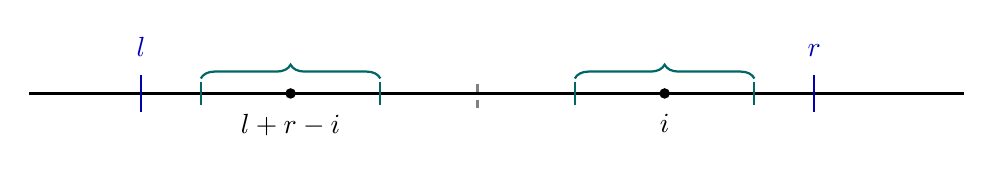
\begin{tikzpicture}[scale=0.95]
    \draw[thick] (0, 0) -- (12.5, 0);

    % Границы l и r
    \draw[thick, blue!70!black] (1.5, -0.25) -- (1.5, 0.25) node[above=3pt] {$l$};
    \draw[thick, blue!70!black] (10.5, -0.25) -- (10.5, 0.25) node[above=3pt] {$r$};
    \draw[thick, dashed, gray] (6.0, -0.2) -- (6.0, 0.2);

    % Точки i' и i
    \fill (3.5, 0) circle (2pt) node[below=4pt] {$l + r - i$};
    \fill (8.5, 0) circle (2pt) node[below=4pt] {$i$};

    % Крылья вокруг них
    \draw[thick, teal!80!black] (2.3, -0.15) -- (2.3, 0.15);
    \draw[thick, teal!80!black] (4.7, -0.15) -- (4.7, 0.15);
    \draw[decorate, decoration={brace, amplitude=5pt}, thick, teal!80!black] (2.3, 0.2) -- (4.7, 0.2);

    \draw[thick, teal!80!black] (7.3, -0.15) -- (7.3, 0.15);
    \draw[thick, teal!80!black] (9.7, -0.15) -- (9.7, 0.15);
    \draw[decorate, decoration={brace, amplitude=5pt}, thick, teal!80!black] (7.3, 0.2) -- (9.7, 0.2);
\end{tikzpicture}
\end{center}

Так как весь отрезок $s[l \dots r]$ "--- палиндром, строка вокруг точки $i$ внутри $[l, r]$ совпадает со строкой вокруг точки $l + r - i$ с точностью до разворота. Но разворот палиндрома "--- снова палиндром! Поэтому:
\begin{itemize}
    \item если палиндром с центром в $l + r - i$ и крылом $m[l + r - i]$ целиком помещается внутри отрезка $[l, r]$, то в точке $i$ есть точно такой же палиндром;
    \item если же палиндром из точки $l + r - i$ <<вываливается>> за левую границу $l$, то за пределами $[l, r]$ симметрия уже не гарантируется, и мы обязаны обрубить крыло палиндрома в точке $i$ по правой границе $r$, то есть длиной $r - i + 1$.
\end{itemize}
Таким образом, при $l \le i \le r$ мы получаем гарантированную нижнюю оценку:
\begin{equation}\label{eq:manacher_bound}
    m[i] \ge \min\bigl(m[l + r - i],\; r - i + 1\bigr)
\end{equation}
(а при $i > r$ тривиальная нижняя оценка равна $m[i] = 1$, поскольку один символ всегда образует палиндром длины $1$).

Дальше алгоритм действует в точности как в Z-функции:
\begin{enumerate}
    \item Записываем в $m[i]$ нижнюю оценку ($1$ при $i > r$ или минимум \eqref{eq:manacher_bound} при $l \le i \le r$).
    \item Пытаемся наивно увеличить $m[i]$ в цикле \texttt{while}: пока мы не вышли за границы строки и символы слева и справа от текущего палиндрома совпадают ($s[i - m[i]] = s[i + m[i]]$), делаем \texttt{++m[i]}.
    \item В конце шага, если правая граница найденного палиндрома $i + m[i] - 1$ оказалась больше $r$, обновляем $l = i - m[i] + 1$ и $r = i + m[i] - 1$.
\end{enumerate}

\begin{lstlisting}
// $s$ "--- строка с уже вставленными символами '\#'
int n = s.size();
vector<int> m(n, 1);
int l = -1, r = -1;
for (int i = 0; i < n; ++i) {
    if (l <= i && i <= r) {
        m[i] = min(m[l + r - i], r - i + 1);
    }
    while (i - m[i] >= 0 && i + m[i] < n && s[i - m[i]] == s[i + m[i]]) {
        ++m[i];
    }
    if (i + m[i] - 1 > r) {
        l = i - m[i] + 1;
        r = i + m[i] - 1;
    }
}
\end{lstlisting}

\begin{theorem}
    Алгоритм Манакера работает за линейное время $O(n)$.
\end{theorem}

\begin{proof}
    Доказательство дословно повторяет анализ Z-функции: следим за правой границей $r$. В цикл \texttt{while} мы заходим только тогда, когда либо $i > r$, либо $i \le r$ и минимум в \eqref{eq:manacher_bound} реализовался на $r - i + 1$. В обоих случаях каждая успешная итерация цикла \texttt{while} расширяет текущий палиндром правее позиции $r$ и увеличивает новое значение $r$ ровно на единицу. Поскольку $r < n$ и $r$ не убывает, цикл \texttt{while} выполнит не более $n$ итераций за всё время работы алгоритма.
\end{proof}
